\FloatBarrier
\section{Data-Oblivious Algorithms}

Data-oblivious algorithms belong to a certain class of algorithms whose method of operation is almost entirely independent of the input data. Such algorithms rely on suitably small atomic operations to modify the data, and in order to maintain independence from the input data, the results of these operations are not known by the algorithm.
 
This restriction naturally makes the development of such algorithms somewhat complicated, and outside of certain examples, most of the field is fairly new. Despite their innate restrictions, this class of algorithms has seen interesting developments in recent years, especially in data-oblivious sorting, where new algorithms have recently been developed following a renewed interest in the field. Along with these developments in data-oblivious sorting, several algorithms that rely heavily on sorting have been adapted to work in a data-oblivious way, due to the high demand for data-oblivious algorithms for distributed secure computations.

Data-oblivious algorithms generally fall into two distinct categories, those that are based on circuits, and those that are randomized.
The circuit-based data-oblivious algorithms model their atomic oblivious operations as gates in a network of data-transporting wires, and achieve data-obliviousness from the fact that this network is fixed, and no change in the ordering of operations can occur based on the content of the input.
Randomized data-oblivious rely on applying their atomic oblivious operations in a randomized manner that is completely independent of the input, and use this fact to achieve data-obviousness, but often cannot be guaranteed to succeed.

It should be noted that the size of the atomic oblivious component can vary widely between applications. The components used in problems concerning  sorting will rarely be sufficient for graph algorithms, and vice versa. Choosing the right size of the data-dependent components depends highly on the context of their use. The atomic operations can vary from simple bitwise or arithmetic operations, to putting two elements in the correct order, and might even consist of sorting a chunk of the input.

Unfortunately, few experiments have been done on the actual performance of these data-oblivious algorithms, which leaves them in a fairly sad state when it comes to implementation details. However, this thesis will provide real-world measurements to alleviate this issue.

\subsection{Motivations for Using Data-Oblivious Algorithms}

Despite their complications, data-oblivious algorithms have several interesting properties that make them an interesting field of work, and the current development into distributed systems is especially driving a new wave of research in this field.

The main motivations are as follows.

\subsubsection{Integrated circuits}

Since any deterministic data-oblivious algorithm can be modelled as a network, using the atomic operation as a network component. If the atomic operation is sufficiently simple, this allows for construction of an electrical circuit that performs the operations of the algorithm.
This implies that for any such algorithm, an integrated component can be developed that, for a fixed input size, will compute the exact same output as the original algorithm. The constantly increasing demand for smart devices combined with the decreasing cost of electronics make data-oblivious algorithms obvious targets for usage in such components.
This was a large part of the motivation for early research into sorting networks, as exemplified in~\citeA{SNApplications} and~\citeA{PrattThesis}. 

\subsubsection{Secure multi-party computations}

When developing systems based on the cooperation of several parties that may not wish to disclose the content of their data, oblivious operations become important. Secure multi-party computations often rely on modelling circuits for any operation that is dependent on input data, which means that reducing the size of the input-dependent components is critical.
Luckily, secure multi-party computations schemes already contain good solutions for generating shared random numbers, which makes randomized data-oblivious algorithms a suitable target for such calculations.
In the literature we find this usage in papers such as~~\citeB{ObliviousSet} and~\citeB{GraphGeoOblivious}.


\subsubsection{Outsourced private data}

When storing private information in an outsourced database, one might wish to hide the content stored from curious observers. Fortunately there exist excellent protocols for encrypting such data, but if the algorithms operating on the data changes its data access patterns based on the content of the data, an observer might infer information about what we are trying to hide. Since the sequence of operations of data-oblivious algorithms is only dependent on the input size, we leak no information when performing important computations.
This use of data-oblivious algorithms forms the basis for~\citeB{ObliviousExternal} and~\citeB{ObliviousGraph}.


\subsubsection{Parallel computing}

In some cases, data-oblivious algorithms can be reduced to a circuit network of low depth. Such networks make great targets for parallel computing. The area of parallel computing is in rapid growth due to the difficulty in constructing faster processors, while the amount of cores in most machines grow, and oblivious algorithms make interesting targets for parallel computation. This however requires special considerations in the algorithmic design, in order to maintain low depth to keep synchronization costs at a minimum.
Research into the applications of parallel execution of data-oblivious are often focused on GPU-assisted sorting algorithms, such as those presented in~\citeA{FastGPU} and~\citeA{OddEvenOpenCL}.  

\subsubsection{Operations on external data}

Systems in which latency for data access is high can benefit heavily from data-oblivious algorithms, as such algorithms can perform their entire workload as a series of atomic operations. These operations can be computed based on the size of the data, and shipped to the external controller, who will then be able to perform these operations. This removes any need for waiting for external latency, while still allowing for a great number of algorithms to be applied. It is especially of note, that while the external party will need to perform a great amount of operations, they will each be of low complexity.
Examples of this usage are hard to find, as most research, such as~\citeB{ObliviousExternal} and~\citeB{ObliviousGraph}, focuses on preventing information leakage through analysis of data access patterns. It can be argued that sorting networks, and integrated circuits would also be applicable to this use case. 


\subsection{Data-Oblivious Sorting Algorithms}

Sorting algorithms are among the oldest researched topics of computer science, and given the importance of efficient sorting algorithms in the design of a wide variety of other algorithms, it is natural to apply great weight to the topic of data-oblivious sorting algorithms.

In the case of data-oblivious sorting, the oblivious atomic operation that is allowed on the input is the \texttt{Compare-Exchange} operation, which, given two indices of the input, will compare the values of the input at the indices and swap them if they are out of order.

The corresponding pseudo-code can be seen in Algorithm~\ref{CompareExchangePseudo}.

\begin{algorithm}
\caption{Compare-Exchange}\label{CompareExchangePseudo}
\begin{algorithmic}[1]
	\Statex $A$: Array input of \texttt{Compare-Exchange} compatible elements
	\Statex $i$: Index of first element of comparison
	\Statex $j$: Index of second element of comparison
\Procedure{Compare-Exchange}{$A, i, j$}
\State $A_{min} \gets \min(A[i], A[j])$
\State $A_{max} \gets \max(A[i], A[j])$
\State $A[\min(i,j)] \gets A_{min}$
\State $A[\max(i,j)] \gets A_{max}$
\EndProcedure
\end{algorithmic}
\end{algorithm}

Note the simplicity of this operation is entirely in line with the data-oblivious mentality of keeping data-dependent components as small as possible, and that unless we explicitly look at the input, we are leaking no information about the results of the procedure.

Using only this operation, a variety of sorting algorithms can be constructed. As mentioned earlier, these algorithms can be divided into randomized and deterministic algorithms.

Data-oblivious sorting is especially well suited for integrated circuits, due to the ease of constructing sorting networks in hardware.
Figure~\ref{fig:bitcompare} shows a simple 1-bit \texttt{Compare-Exchange} circuit. Also, any N-bit \texttt{Compare-Exchange} operation can be constructed from an N-bit comparator and two 2N:N multiplexers, both of which can be easily constructed, or bought ready-made for most small powers of 2.

\begin{figure}
\center
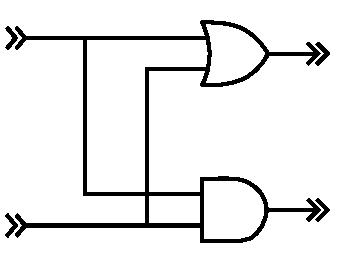
\includegraphics[width= 0.25 \textwidth]{Graphics/1bitCompare.pdf}
\caption{1-bit hardware \texttt{Compare-Exchange}}
\label{fig:bitcompare}
\end{figure}

Sometimes it might be necessary to employ a reverse \texttt{Compare-Exchange} operation, which will swap the elements such that they are in reverse sorted order. Such an operation is obviously just as viable and data-independent as the regular \texttt{Compare-Exchange} operation, but may sometimes give a larger degree of freedom in the description of algorithms.

\subsubsection{Deterministic Data-oblivious Sorting Algorithms}

Deterministic data-oblivious sorting algorithms form a large group of algorithms, though many of them are not known by their data-oblivious qualities, but instead as sorting networks.

\begin{figure}
\center
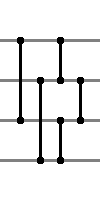
\includegraphics[width= 0.15 \textwidth]{Graphics/network.png}
\caption{4-wire sorting network, equivalent to \texttt{Compare-Exchange} for inputs $(0,2), (1,3), (0,1), (2,3), (1,2)$}
\label{fig:network}
\end{figure}

It is important to note that any fixed sorting network is a data-oblivious sorting algorithm, and can be modelled using \texttt{Compare-Exchange} operations, by performing such an operation for each comparison on the wires of the networks, as seen in Figure\ref{fig:network}. Additionally, any deterministic sorting algorithm depending entirely on \texttt{Compare-Exchange} operations can be viewed as a sorting network that runs a wire for each element of the input, and perform a comparison between wire contents wherever the algorithm performs a \texttt{Compare-Exchange} operation.

Due to their roots in sorting networks, data-oblivious sorting algorithms have a long history, and many algorithms have been developed to perform as sorting networks.

The historical algorithms of Bubble Sort~\citeB{BubbleSort} and the original Shellsort~\citeA{Shellsort} are both examples of simple algorithms that can easily be made data-oblivious by removing any checks for sortedness. This leaves them at their $\Theta(n^2)$ worst-case running time, but makes them easily understandable as data-oblivious algorithms.

Optimal sorting networks have been constructed, running in $\Theta(n \log n)$ time. The most famous of these networks is the AKS sorting network of~\citeA{AKS}, which is widely known, and form the basis of a great deal of research in the sorting networks field. Worth mentioning is also Zig-Zag Sort~\citeA{ZigZag} which is especially interesting due to its simplicity.
These optimal sorting networks are all entirely dependent on the usage of \textepsilon -halvers; a construction that is complicated to produce deterministically, and  has a very high constant factor to their number of comparison. The problem of constructing \textepsilon -halvers makes these optimal sorting networks of little use in practical implementations.

Pratt presents a more efficient variant of Shellsort in his thesis~\citeA{PrattThesis}, that is not only $\Theta(n \log^2 n)$ in the amount of comparisons, but also easily translates into a sorting network. The main idea of Pratt's variant Shellsort, is using a special $\Theta(\log^2 n)$-length jump sequence, instead of the old-fashioned geometric sequences that are often used in Shellsort.

A final interesting family of sorting networks are the algorithms stemming from Batcher's paper on sorting networks~\citeA{SNApplications}, known as Bitonic Sort and Odd-Even Mergesort, along with the Pairwise Sorting Network~\citeA{PairwiseSorting}. These sorting networks achieve sorting at $\Theta(n \log^2 n)$ comparisons, while maintaining a $\Theta(\log^2 n)$ depth, and are simple enough to be implemented on standard hardware, though their asymptotical complexity makes them somewhat lacking when compared to non-oblivious sorting algorithms.

\subsubsection{Randomized Data-Oblivious Sorting Algorithms}

Randomized data-oblivious sorting algorithms are a fairly new development, primarily introduced by \citeA{RandShellSort} and \citeA{AnnealingSort}, but an interesting one. Unfortunately, the list of algorithms performing data-oblivious sorting using a randomized sequence of \texttt{Compare-Exchange} is somewhat short. They are however useful due to the fact that they are simple in their method of operations.

From~\citeA{AnnealingSort} we get Spin-the-bottle Sort and Annealing Sort. The former of which is a $\Theta(n^2 \log n)$ data-oblivious sorting algorithm, of interest only in setting the stage for Annealing Sort, which will with very high probability, sort any given input obliviously in $\Theta(n \log n)$ time.
It is worth noting that the amount of comparisons performed by Annealing Sort has a high constant coefficient if the values given in~\citeA{AnnealingSort} are used, but this could easily be the result of overly pessimistic analysis, as is also the case of~\citeA{RandShellSort}.

A variant of Shellsort, called Shaker Sort is presented in~\citeA{ShakerSort}, and can be implemented as a $\Theta(n \log n)$ sorting network.
Shaker Sort's main deviance from Shellsort is replacing the subsequence sorting with so-called \emph{h-shakes}, which are linear-complexity applications of \texttt{Compare-Exchange} operations up and down the subsequence. Despite having certain bad input permutations, Shaker Sort shows great potential in sorting randomized input data.
By shuffling the input sequence to break up inputs that have been carefully constructed as adversary inputs, we can obtain a randomized variant of Shaker Sort, that  will show excellent performance characteristics, though this requires data-oblivious constructs beyond the \texttt{Compare-Exchange} operation, and will make the algorithm unsuitable for construction as a pure sorting network.

Finally, from~\citeA{RandShellSort} we get Randomized Shellsort, an algorithm that will sort with very high probability in $\Theta(n \log n)$ time by performing \texttt{Compare-Exchange} among random matching pairings taken from regions of the input in regions of sizes matching the subsequence jumps of the original Shellsort algorithm.

Sorting networks can be constructed from randomized data-oblivious algorithms by recording the sequence of operations the algorithm would perform, and constructing the corresponding network. This will lead to networks that use the same amount of comparator components as the amount of \texttt{Compare-Exchange} operations used in algorithm, but the network might not adapt well in terms of depth.

\subsubsection{Algorithms Tabular}

Since the previous subsection includes a great amount of different algorithms, we here present them in short tabular form, as a quick reference sheet.
The table in question is Table~\ref{BigAlgTable}.
\begin{table}[!h]
\begin{adjustwidth}{-.5in}{-.5in}
\centering
\begin{tabular}{|c c c c|}
\hline
Name & Source & Running Time & Keywords \\\hline
Bubble Sort & ~\citeB{BubbleSort} & $\Theta(n^2)$ & Simple \\
Shellsort & ~\citeA{Shellsort} & varies & Customizable, Well-researched \\
AKS Sorting Network & ~\citeA{AKS} & $\Theta(n \log n)$ & Optimal, Theoretical, Depth-optimal \\
Zig-Zag Sort & ~\citeA{ZigZag} & $\Theta(n \log n)$ & Optimal \\
Pratt's Shellsort & ~\citeA{PrattThesis} & $\Theta(n \log^2 n)$ & Shellsort-based\\
Bitonic Sort & ~\citeA{SNApplications} & $\Theta(n \log^2 n)$ & Well-known, Practical \\
Odd-Even Mergesort & ~\citeA{SNApplications} & $\Theta(n \log^2 n)$ & Merge Sort \\
Pairwise Sorting Network & ~\citeA{PairwiseSorting} &  \textcolor{red}{$\Theta(n \log^2 n)$} & Simple \\
Spin-the-bottle Sort & ~\citeA{AnnealingSort} & $\Theta(n^2 \log n)$ & Randomized, Unused \\
Annealing Sort & ~\citeA{AnnealingSort} & $\Theta(n \log n)$ & Randomized, Impractical \\
Shaker Sort & ~\citeA{ShakerSort} & $\Theta(n \log n)$ & Shellsort-Based, Possible~Randomization \\
Randomized Shellsort & ~\citeA{RandShellSort} & $\Theta(n \log n)$ & Randomized, Shellsort-based \\\hline
\end{tabular}
\end{adjustwidth}
\caption{Table of algorithms}
\label{BigAlgTable}
\end{table}

\subsection{Other Data-Oblivous Algorithms}

Most of the work done in the field of data-oblivious algorithms concerns itself with the sorting of numbers. This stems from the existence of sorting networks as an already established field, and the nature of sorting giving itself easily to the concept of data obliviousness. There are however other classes of data-oblivious algorithms, though they are scarce, and not always easily adaptable to modern hardware.

In order to construct a probabilistic sorting network probabilistic data-oblivious algorithms for merging and selection are presented in~\citeB{ProbNetworks}. Data-oblivious merging is already made possible by~\citeA{SNApplications} in $\Theta(n \log n)$ time, and this running time is not asymptotically improved, but the paper shows that the problem of data-oblivious selection is faster than any known solution to data-oblivious sorting.

Selection, along with compaction and sorting, is also explored in~\citeB{ObliviousExternal} using the external memory model, as a means to provide a solution for such problems, when one must perform privacy-preserving computations on externally located data. Note that for data-oblivious algorithms in the external memory model, any computations are allowed in internal memory, and only the accesses to external memory needs to be kept oblivious.

A great number of set operations are shown to be computable in an oblivious and privacy-preserving manner in~\citeB{ObliviousSet}. These algorithms can become the fundamental building blocks for later algorithms, and are therefore of great significance to the field of data-oblivious algorithms.

Several crucial graph algorithms, namely breath-first search, single-source shortest distance, maximum flow and minimum spanning tree, have efficient data-oblivious algorithms for dense graphs presented in~\citeB{ObliviousGraph}. These are especially interesting, as they venture far from the well-known area of sorting, and can be useful for doing multi-party network routing computations, where one might wish to keep the algorithm oblivious due to privacy concerns.

A number of geometric problems, convex hull, quadtree construction, closest pair and all-nearest-neighbours have data-oblivious solutions presented in~\citeB{GraphGeoOblivious}. These serve as useful building blocks for applications that are privacy-preserving, distributed and location-aware. 

Finally, it should be noted that the existence of the concept \emph{Oblivious RAM} is often mentioned in the data-oblivious literature. Oblivious RAM is an ingenious concept originating from~\citeB{ObliviousRam} that allows the execution of arbitrary algorithms in a manner that prevents an adversary from obtaining useful information about the input from the memory accesses of the algorithm. This is especially useful for privacy-preserving computations, but imposes a non-constant overhead on the complexity of the program, which means that the development of optimal data-oblivious algorithms is still relevant.